\section{Shock-tubes}

In this section, we focus on simulation of soot formation in shock-tubes using the constant volume reactor of omnisoot, and compare species mole fraction and soot yield and morphology (if available) with benchmark measurements. Figure~\ref{fig:shocktubeschem} (left pane) illustrates the schematics of a shock-tube along with the idealized wave diagram. Shock-tubes are typically designed as a several meter long cylindrical tube separated by thin diaphragm into a smaller driver section filled a high pressure inert gas, and a longer driven section with diluted reactants. When the diaphragm is ruptured, the first shock wave propagates through the reactant mixture. The front shock compresses the reactants adiabatically raising the temperature and pressure throughout the shock-tube from $\mathrm{T_1}$, $\mathrm{P_1}$ to $\mathrm{T_2}$, $\mathrm{P_2}$. The passage of the reflected shock from the end wall heats up the reactants for the second time reaching $\mathrm{T_5}$, $\mathrm{P_5}$. Figure~\ref{fig:shocktubeschem} (right pane) shows the first and second jump in pressure due to the front and reflected shocks, respectively, and the variation in soot volume fraction during the pyrolysis of 0.03\% benzene in Ar. The reflected shock creates a nearly still mixture with a constant temperature and pressure (as shown in left pane of Figure~\ref{fig:shocktubeschem}) which provides an ideal condition for kinetic studies and rate constant investigations~\citep{kee2017chemically}. Therefore, the use of a shock tube provides a unique opportunity for investigating the kinetics of soot formation from fuels and at various temperatures, pressures and concentrations.

However, the processes investigated in shock tubes are limited to short residence times usually 1-3 ms, so they can only be used to study early stages of soot formation such as inception and surface growth, and not for processes occurring at longer residence times such as coagulation and carbonization. Note that the residence time is calculated after the passage of reflected shock. There is a delay in the increase of volume fraction known as induction time, $\mathrm{\tau_{ind}}$. There has been a lot of research in the literature focused on induction time (similarly on ignition delay time) in shock tubes~\citep{fussey1978shock}, but it is not the focus of this work. Instead, here we mainly investigate the species concentrations and soot characteristics during the pyrolysis of hydrocarbons, especially methane, at atmospheric and higher pressure which can be used for the design and optimization of carbon black in plasma reactors~\citep{fulcheri2023energy}. 

First, the pyrolysis of 5\% and 10\% $\mathrm{CH_4}$ diluted with Ar is investigated for the post-shock temperature range of 1800-3000 K and the pressure range of 4.7-7.1 bar. We assume the pressure linearly increase by temperature across the simulation cases. The obtained soot yields by were compared with the soot yield measured by \citet{agafonov2016unified} using a dual-beam absorption–emission technique. \citet{agafonov2016unified} reported yield$\times$E(m) at $\mathrm{\lambda}$=632~nm, and yield data was retrieved using E(m)=0.37 suggested therein. 




% run the shock-tube with other mechanisms and include the results in the Appendix

\begin{figure}[!htbp]
	\centering
	\begin{subfigure}[t]{0.4\textwidth}
		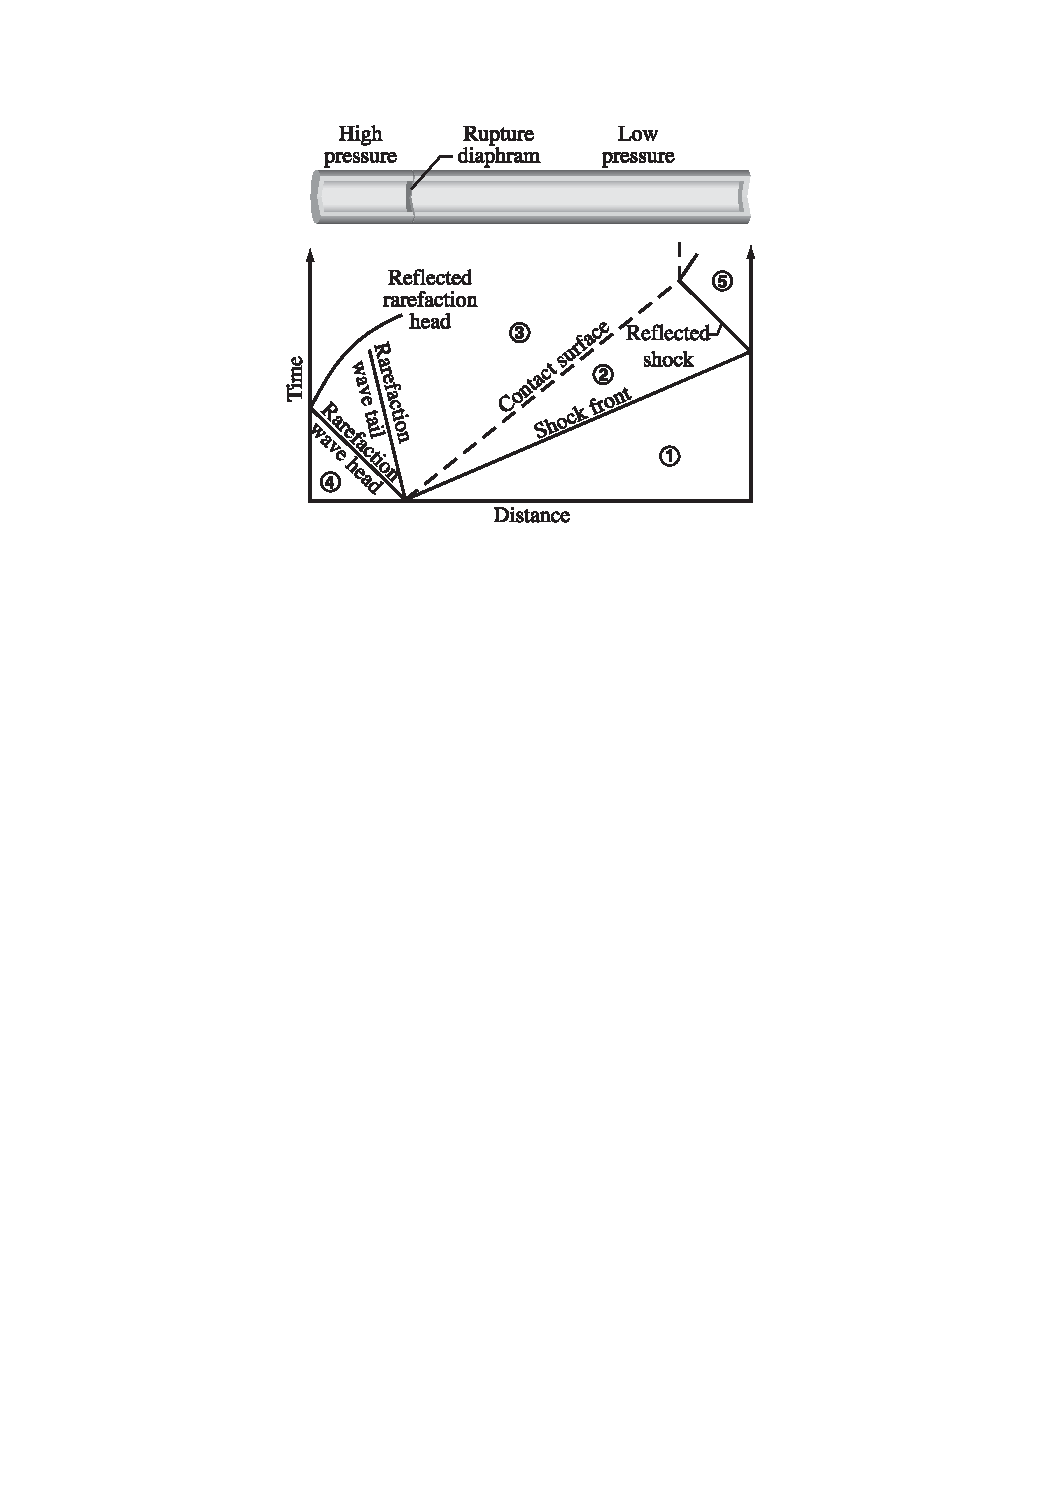
\includegraphics[width=1\textwidth]{Figures/Results/Shocktube/schematics.pdf}
	\end{subfigure}
	\begin{subfigure}[t]{0.4\textwidth}
	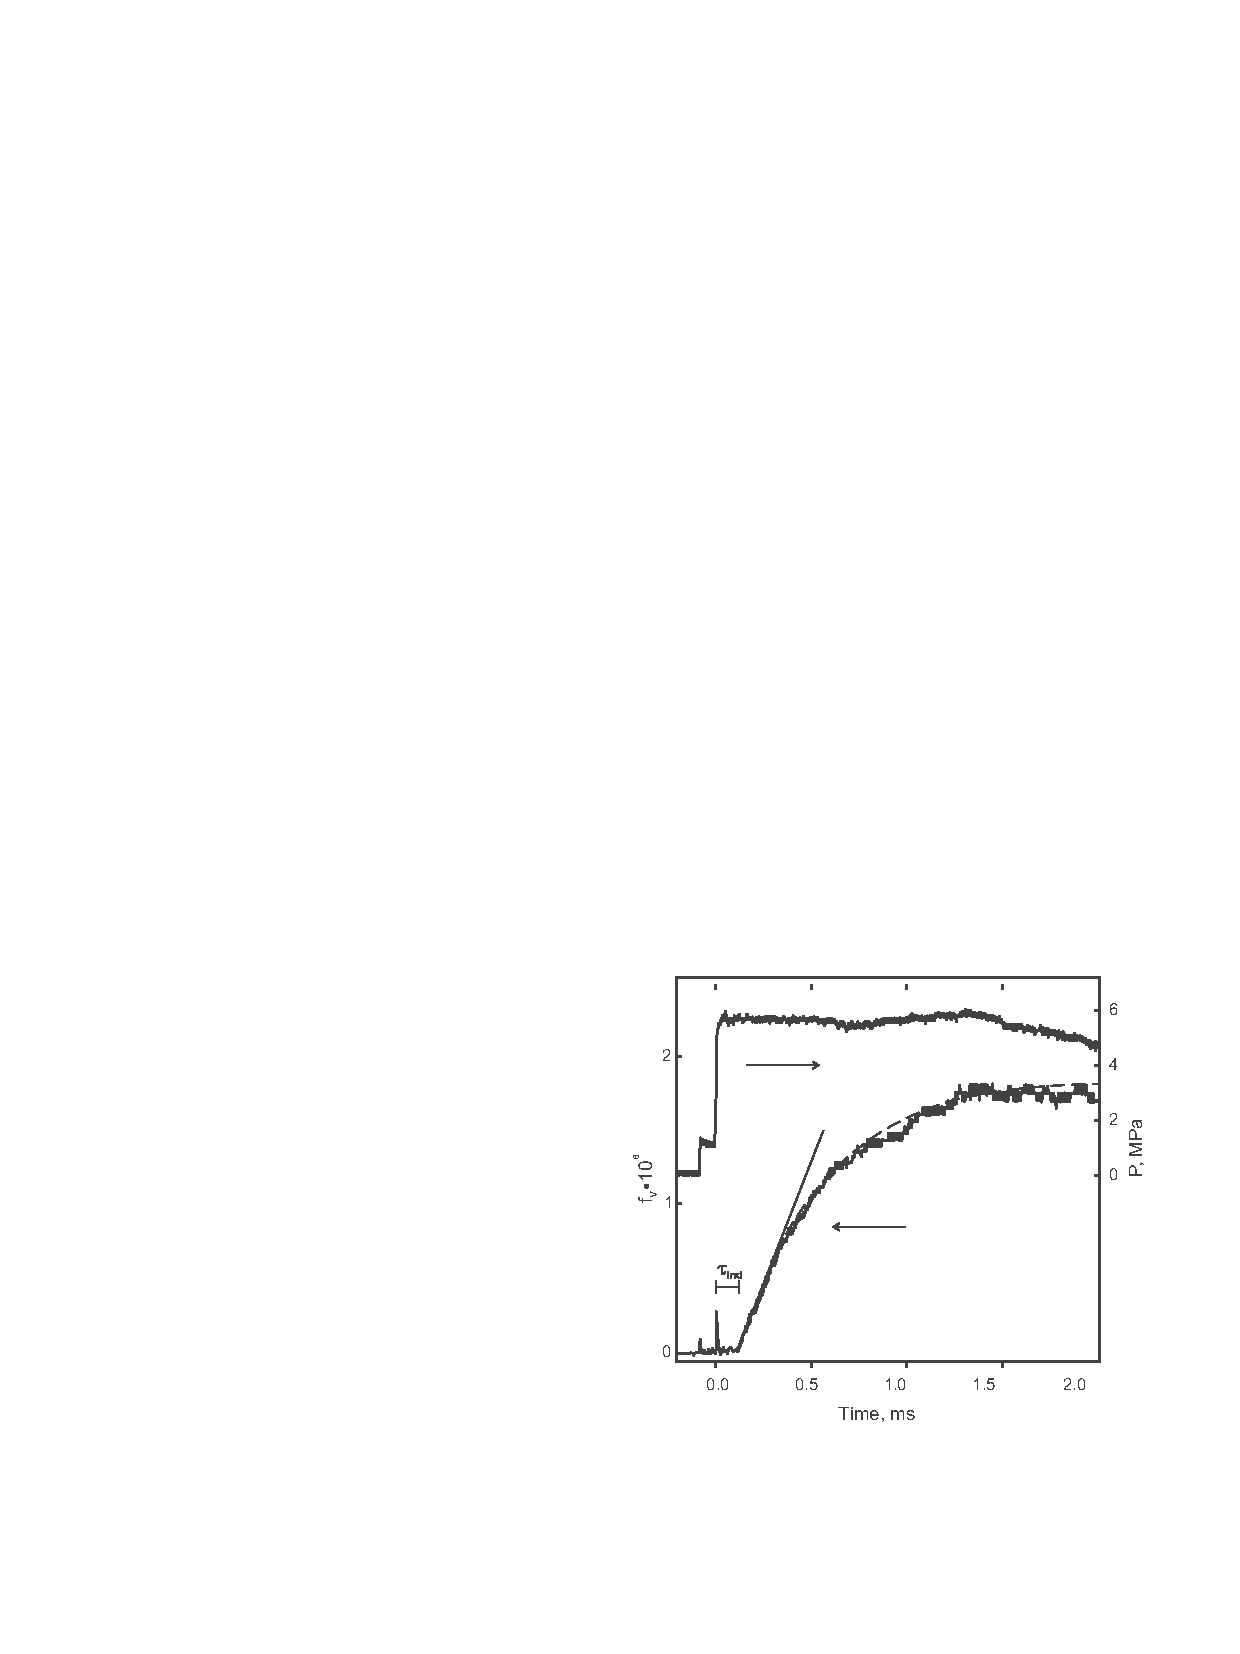
\includegraphics[width=1\textwidth]{Figures/Results/Shocktube/pfv_sample_shocktube.pdf}
	\end{subfigure}
	\caption{The schematics of a shock-tube and the idealized shockwave diagram(left pane reprinted from ~\citet{kee2017chemically}) and the variation of soot volume fraction measured by the extinction record at 633 nm and the pressure profile behind the reflected shock wave in a mixture 0.03\% benzene in Ar at T = 1890 K(right pane reprinted from ~\citet{karasevich1994soot})}
	\label{fig:shocktubeschem}
\end{figure}

Figure~\ref{fig:shocktubeyield} depicts soot yield (SY) at t=1.5 ms for 5\% and 10\% $\mathrm{CH_4}$ over the temperature range of 1800-3000 K using MPBM and SPBM and different inception model and Caltech~\citep{blanquart2009chemical} mechanism. Note that, the simulations were also performed using ABF~\citep{appel2000kinetic} and KAUST~\cite{wang2013pah} mechanisms, and the results were included in Appendix\hl{****}. The soot yield predictions exhibit a close agreement with measurements~\citep{agafonov2016unified} considering the uncertainties in residence time from experiments. The model also successfully captures the bell-shape dependence of soot yield on temperature that has been observed in a variety of hydrocarbons in shock tube~\citep{kellerer1996soot,knorre1996soot}. The particle dynamics model has minimal effect on the predicted soot yield. In the vicinity of peak soot yield, SPBM results in slightly lower yield than MPBM, but they are indistinguishable in the rest of the temperature range. 

%The minor difference between MPBM and SPBM is due to the short residence time (t=1.5 ms) where inception and surface growth are dominant leading to low polydispersity and relatively small agglomerates. 
In \%5 $\mathrm{CH_4}$, the SY peak temperature obtained from the model is slightly shifted towards higher temperatures (2300 K$<T_{peak}<$2400 K) compared to the measurements $T_{peak}=$2200 K. There are noticeable differences in the behavior of PAH growth model depending on the shock-tube initial temperature. When T$<$2100 K, Reactive Dimerization and EBridge Formation have the highest and lowest soot yield, respectively with Dimer Coalescence predicting soot yields that always falls between Reactive and Irreversible Dimerization. However, The soot yield of EBridge Formation rapidly rises with temperature and exceeds that of Reactive Dimerization and stays higher for the rest of temperature range.

The SY noticeably increases for higher initial $\mathrm{CH_4}$ mole fraction of \%10 because more PAH and $\mathrm{C_2H_2}$ are formed leading to stronger carbon conversion rate to soot via inception and surface growth. The peak SY obtained from the model occurs in a higher temperature range 2600-2700 K compared to \%5 $\mathrm{CH_4}$. Soot yield trends can be better understood by examining carbon mass fraction of species directly contributing to soot mass. Figure~\ref{fig:shocktubeAAAA} depicts the bell-shape distribution of the carbon mass fraction of soot precursors (A2, A2R5, A3, and A4) over the studied temperature range. In low (T=1800 K) and high (T=2300 K) end of distribution, a low amount of precursors are formed resulting in low inception rates, particle number concentration and surface growth sites that reduces the soot yield. Additionally, \%10$\mathrm{CH_4}$ has a wider spread with peaks at higher temperature compared to \%10$\mathrm{CH_4}$ which explains the shift in peak yield temperature in Figure~\ref{fig:shocktubeyield}. The effect of particle dynamics model is only noticeable in Reactive Dimerization where SPBM results in higher precursor CMF (lower consumption) due to its lower PAH adsorption rates. %Should discuss why the difference only appears in RD not the others


\begin{figure}[H]
	\centering
	\begin{subfigure}[t]{0.4\textwidth}
		\begin{tikzpicture}
			\draw (0, 0) node[inner sep=0] 	{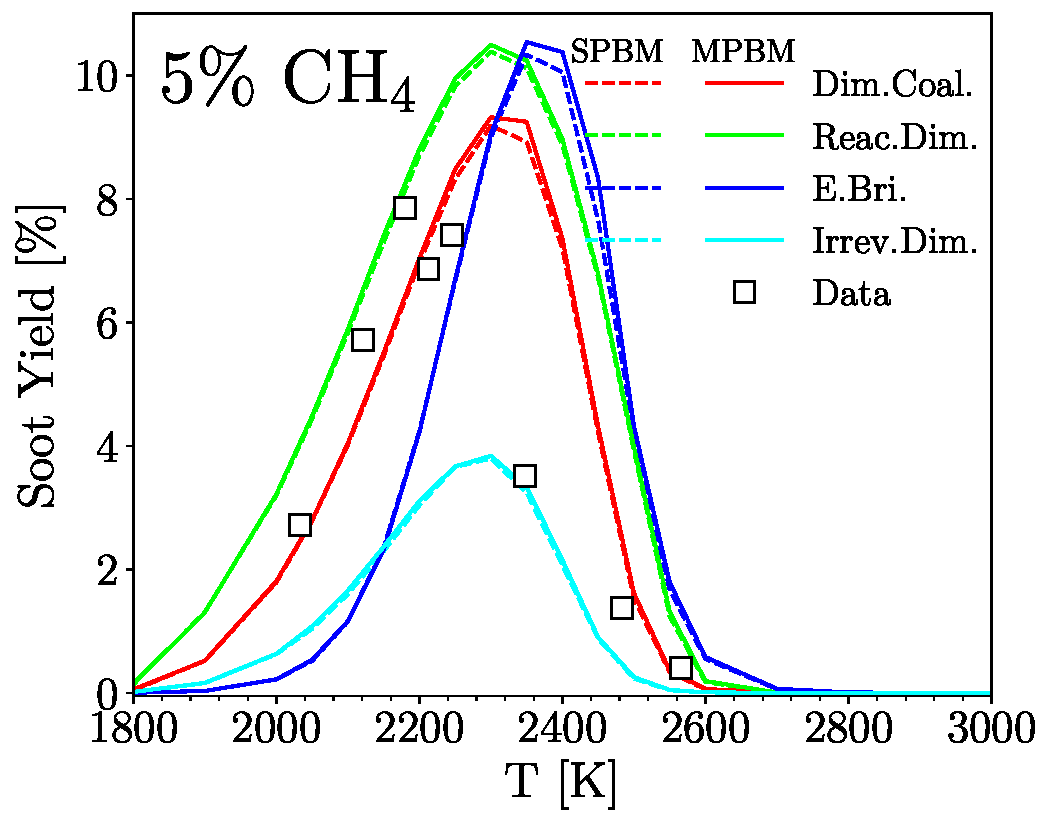
\includegraphics[width=1\textwidth]{Figures/Results/Shocktube/Agafonov2016/5CH4/carbon_yield.pdf}};
			\draw (2.44, 0.68) node {\tiny{\cite{agafonov2016unified}}};
		\end{tikzpicture}
	\end{subfigure}
	\begin{subfigure}[t]{0.4\textwidth}
	\begin{tikzpicture}
		\draw (0, 0) node[inner sep=0] 	{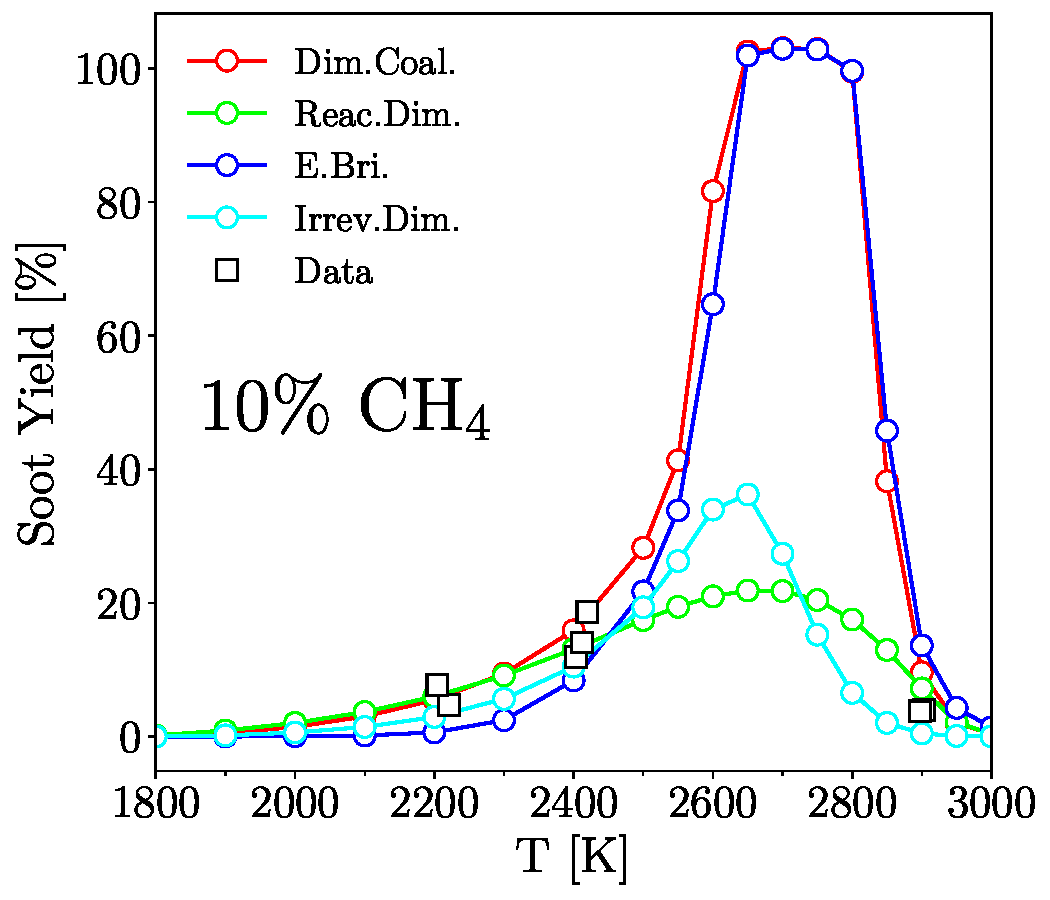
\includegraphics[width=1\textwidth]{Figures/Results/Shocktube/Agafonov2016/10CH4/carbon_yield.pdf}};
		\draw (0.29, -0.33) node {\tiny{\cite{agafonov2016unified}}};
	\end{tikzpicture}
	\end{subfigure}
	\caption{The temperature dependence of soot yield during pyrolysis of 5\%~$\mathrm{CH_4}$-Ar (left pane) and 10\%~$\mathrm{CH_4}$-Ar (right pane) at $\mathrm{P}$ = 4.5–6.7 bar obtained using Caltech mechanism and different inception models compared with measurements at 1.5ms~\cite{agafonov2016unified} where the absorption funtion of E(m)=0.37 is used to estimate soot yield.}
	\label{fig:shocktubeyield} 
\end{figure}


\begin{figure}[H]
	\centering
	\begin{subfigure}[t]{0.4\textwidth}
		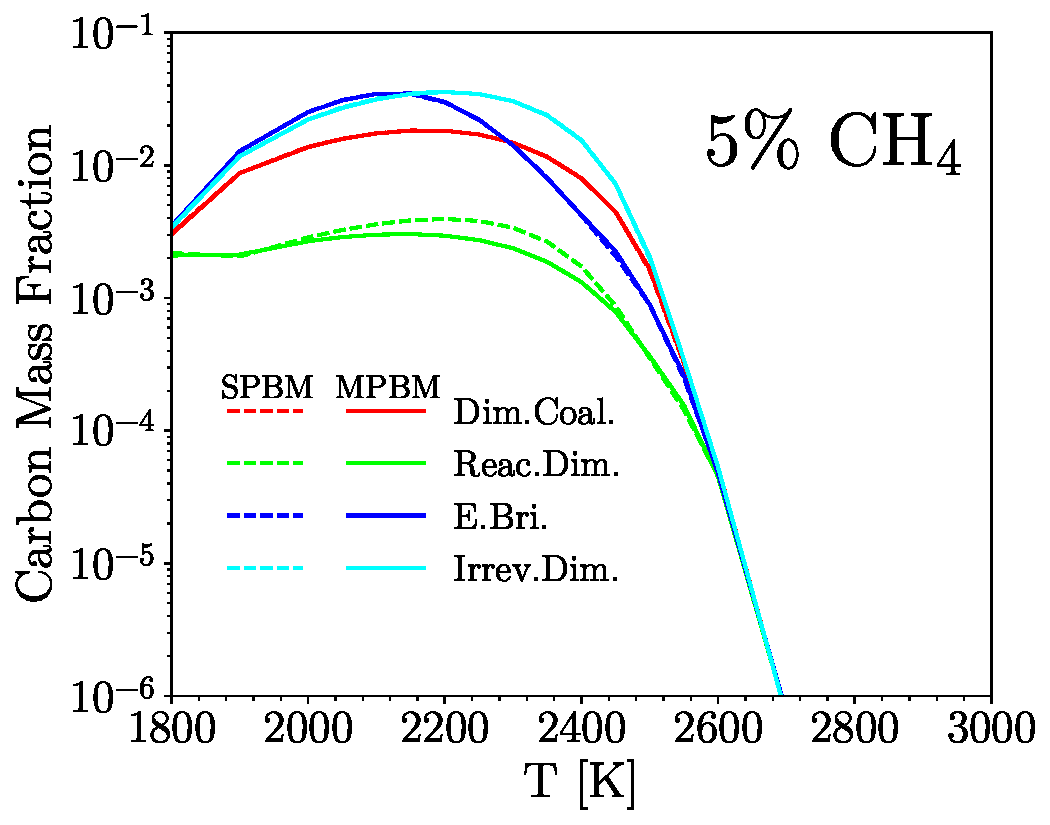
\includegraphics[width=1\textwidth]{Figures/Results/Shocktube/Agafonov2016/5CH4/AAAA.pdf}
	\end{subfigure}
	\begin{subfigure}[t]{0.4\textwidth}
		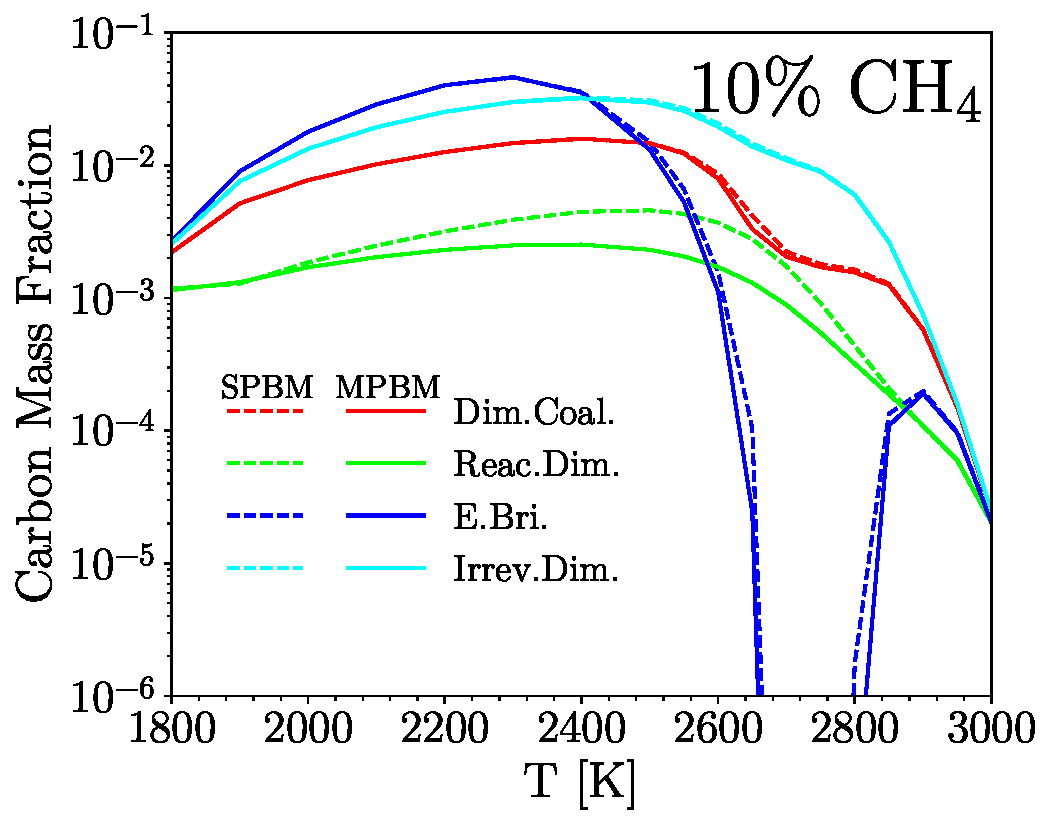
\includegraphics[width=1\textwidth]{Figures/Results/Shocktube/Agafonov2016/10CH4/AAAA.pdf}
	\end{subfigure}
	\caption{The temperature dependence of carbon mass fraction of soot precursors (A2, A2R5, A3, and A4) combined during pyrolysis of 5\%~$\mathrm{CH_4}$-Ar (left pane) and 10\%~$\mathrm{CH_4}$-Ar (right pane) at $\mathrm{P}$ = 4.5–6.7 bar obtained using Caltech mechanism and different inception models at t=1.5 ms}
	\label{fig:shocktubeAAAA} 
\end{figure}

EBridge Formation exhibits a similar behavior in \%10 $\mathrm{CH_4}$ simulations where it starts with the lowest SY at T$<$2500 K and then quickly increases reaching its peak at 100\% which is significantly larger that other PAH growth models. The remarkable drop in carbon mass fraction of precursors with EBridge Formation corresponds to \%100 yield meaning that all gaseous carbon including the precursors are directed towards soot particles.The higher precursor CMF with Irreversible Dimerization near the peak yield temperature region (2200-2400 K for \%5 $\mathrm{CH_4}$ and 2600-2800 K for \%10 $\mathrm{CH_4}$) indicates less consumption of precursors via inception and PAH adsorption.

Figure~\ref{fig:shocktubeC2H2} shows the CMF of $\mathrm{C_2H_2}$ that has an overall increasing trend in the temperature range, but it reaches a plateau for \%5 $\mathrm{CH_4}$. There is also a remarkable drop in $\mathrm{C_2H_2}$ CMF in 2600-2800 K due to strong mass growth rate of soot particles that drains $\mathrm{C_2H_2}$ from the gas mixture leading to high soot yield $\approxeq 100\%$. 


\begin{figure}[!htbp]
	\centering
	\begin{subfigure}[t]{0.4\textwidth}
		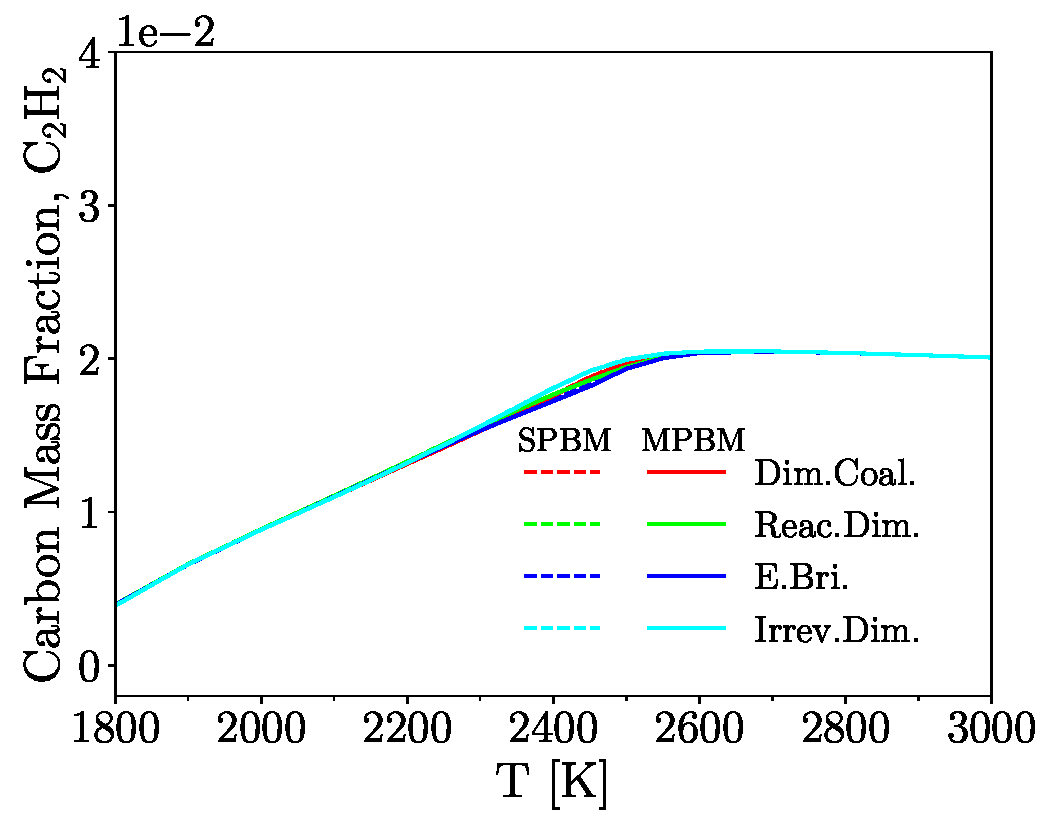
\includegraphics[width=1\textwidth]{Figures/Results/Shocktube/Agafonov2016/5CH4/C2H2.pdf}
	\end{subfigure}
	\begin{subfigure}[t]{0.4\textwidth}
		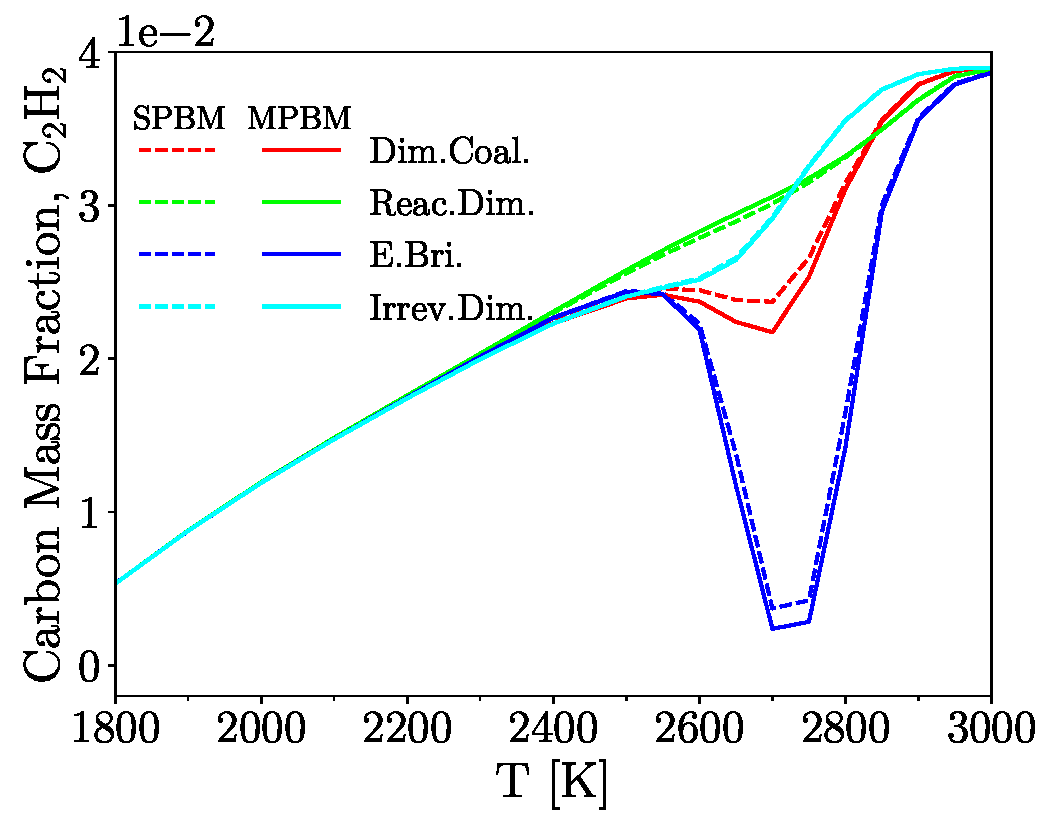
\includegraphics[width=1\textwidth]{Figures/Results/Shocktube/Agafonov2016/10CH4/C2H2.pdf}
	\end{subfigure}
	\caption{The temperature dependence of carbon mass fraction of $\mathrm{C_2H_2}$ during pyrolysis of 5\%~$\mathrm{CH_4}$-Ar (left pane) and 10\%~$\mathrm{CH_4}$-Ar (right pane) at $\mathrm{P}$ = 4.5–6.7 bar obtained using Caltech mechanism and different inception models at t=1.5 ms}
	\label{fig:shocktubeC2H2} 
\end{figure}

Although soot yield, and precursor and acetylene CMF are not sensitive to particle dynamics model, there is a significant difference in agglomerate morphology between SPBM and MPBM predictions. Fig.~\ref{fig:shocktubenp} shows the average number of primary particles per agglomerate, which is larger for SPBM by the maximum factor of 5 for EBridge Formation and Dimer Coalescence in 10\%~$\mathrm{CH_4}$. SPBM predicts larger agglomerates due to accounting for polydispersity of particles that results in higher overall collision rate and faster growth by coagulation. $\mathrm{n_p}$ follows a bell-shape trend similar to soot yield (Fig.~\ref{fig:shocktubeyield}). The $\mathrm{n_p}$ values and the difference between the particle dynamics models reaches their maximum in 2200-2400 K for \%5 $\mathrm{CH_4}$ and 2600-2800 K for \%10 $\mathrm{CH_4}$ because of a stronger inception flux leading to larger number concentration of particles and higher coagulation rate. $\mathrm{n_p}$ is larger for Dimer Coalescence and EBridge Formation reaching the maximum of nearly 100 and 1000 in \%5 and \%10 $\mathrm{CH_4}$, respectively using SPBM. The effect of particle dynamics is minimum for Reactive and Irreversible Dimerization at 5\%~$\mathrm{CH_4}$ over the whole temperature range. 

Fig.\ref{fig:shocktubesigma} shows the standard geometric deviation of mobility diameter, $\mathrm{\sigma_{g}}$ obtained by SPBM that reaches the maximum of 5 and 10 for \%5 and \%10 $\mathrm{CH_4}$, respectively indicating a significant degree of polydispersity in the generated particles at t=1.5ms.

%plot sigma in time to see how it changes and why the sigma values are so large + compare sigma with values from the flame

\begin{figure}[H]
	\centering
	\begin{subfigure}[t]{0.4\textwidth}
		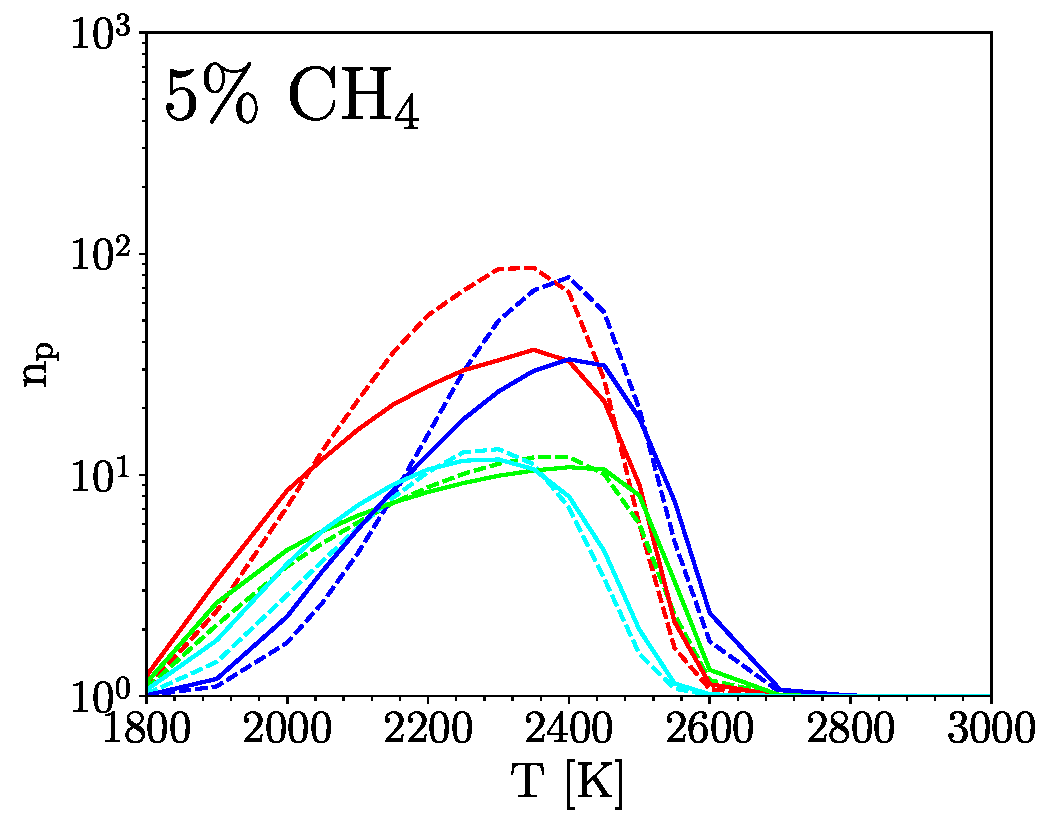
\includegraphics[width=1\textwidth]{Figures/Results/Shocktube/Agafonov2016/5CH4/n_p.pdf}
	\end{subfigure}
	\begin{subfigure}[t]{0.4\textwidth}
		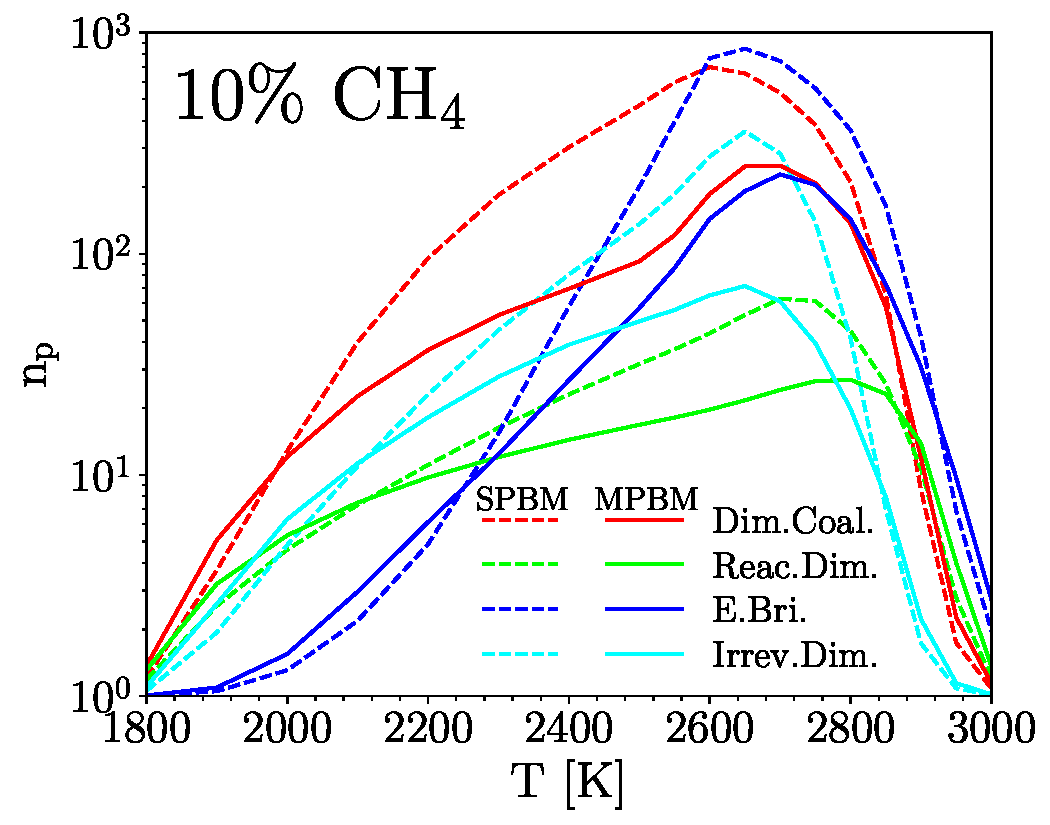
\includegraphics[width=1\textwidth]{Figures/Results/Shocktube/Agafonov2016/10CH4/n_p.pdf}
	\end{subfigure}
	\caption{The temperature dependence of average number of primary particle per agglomerate, $\mathrm{n_p}$ during pyrolysis of 5\%~$\mathrm{CH_4}$-Ar (left pane) and 10\%~$\mathrm{CH_4}$-Ar (right pane) at $\mathrm{P}$ = 4.5–6.7 bar obtained using Caltech mechanism and different inception models at t=1.5 ms}
	\label{fig:shocktubenp} 
\end{figure}

\begin{figure}[H]
	\centering
	\begin{subfigure}[t]{0.4\textwidth}
		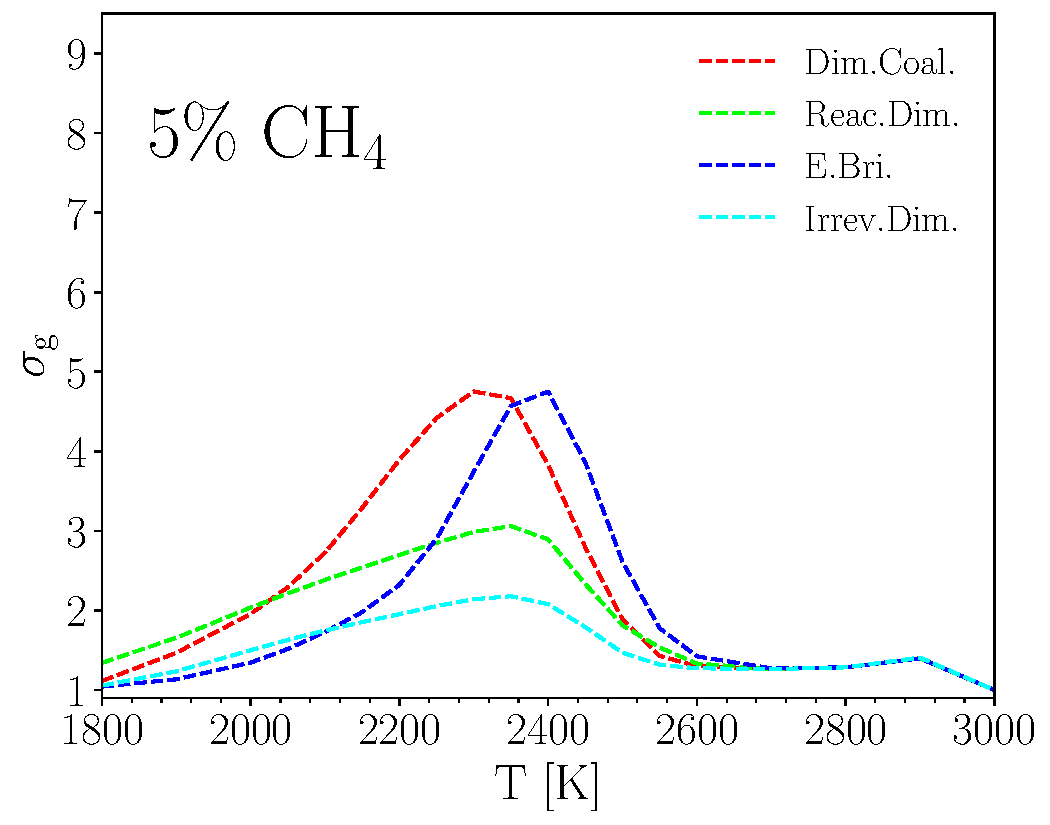
\includegraphics[width=1\textwidth]{Figures/Results/Shocktube/Agafonov2016/5CH4/sigma.pdf}
	\end{subfigure}
	\begin{subfigure}[t]{0.4\textwidth}
		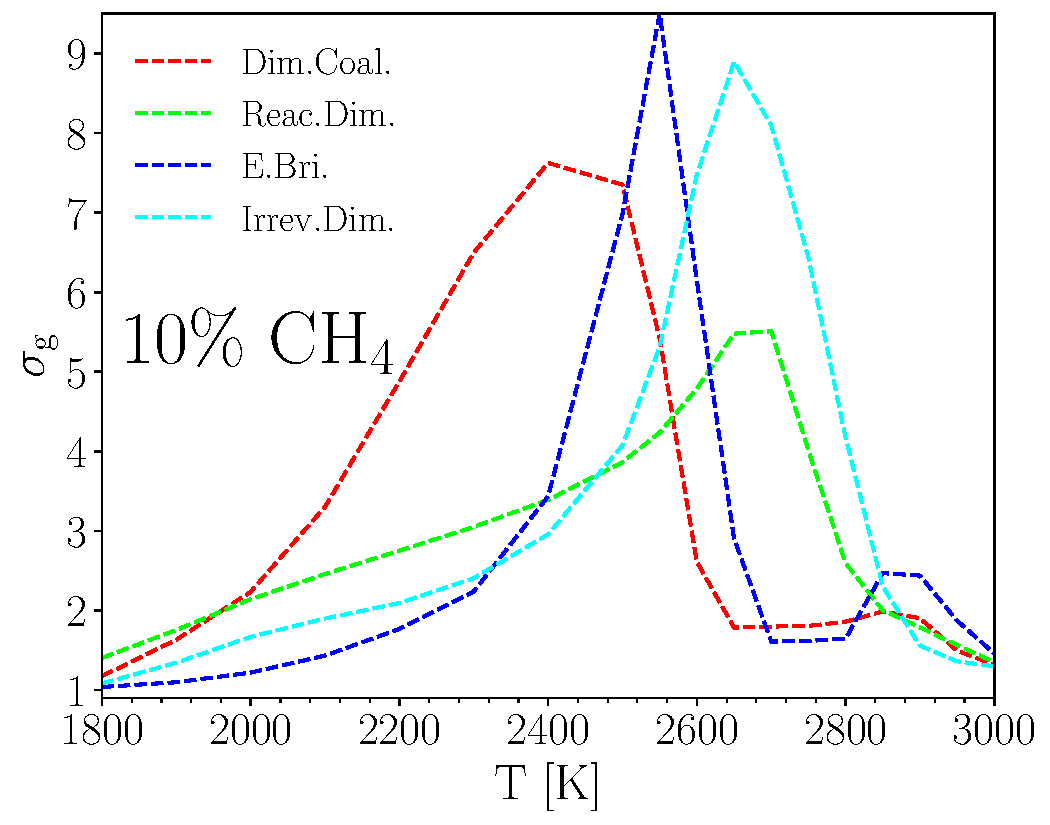
\includegraphics[width=1\textwidth]{Figures/Results/Shocktube/Agafonov2016/10CH4/sigma.pdf}
	\end{subfigure}
	\caption{The time variation of standard geometric deviation of mobility diameter, $\mathrm{\sigma_{g}}$ during pyrolysis of 5\%~$\mathrm{CH_4}$-Ar (left pane) and 10\%~$\mathrm{CH_4}$-Ar (right pane) at $\mathrm{P}$ = 4.5–6.7 bar obtained using Caltech mechanism and different inception models at t=1.5 ms}
\label{fig:shocktubesigma} 
\end{figure}

The $\mathrm{\sigma_{g}}$ values from the SMPS measurements of soot particles at t$\approx$=45ms in a benchmark burner-stabilized premixed are close to 1.1, which is significantly lower than values observed here. So, the evolution of $\mathrm{\sigma_{g}}$ in the studied shock tube is examined in an extended time frame up to 4 msf for 10\%~$\mathrm{CH_4}$ at T=2500 and 2700 K. As shown in Fig.\ref{fig:shocktubesigmatime}, for all PAH growth models $\mathrm{\sigma_{g}}$ rises in the beginning due to simultaneous inception and coagulation that increases polydispersity and rapidly drops and approaches 1.5 before t=3ms when coagulation becomes dominant and inception weaken due to consumption of precursors by PAH adsorption and HACA.


\begin{figure}[H]
	\centering
	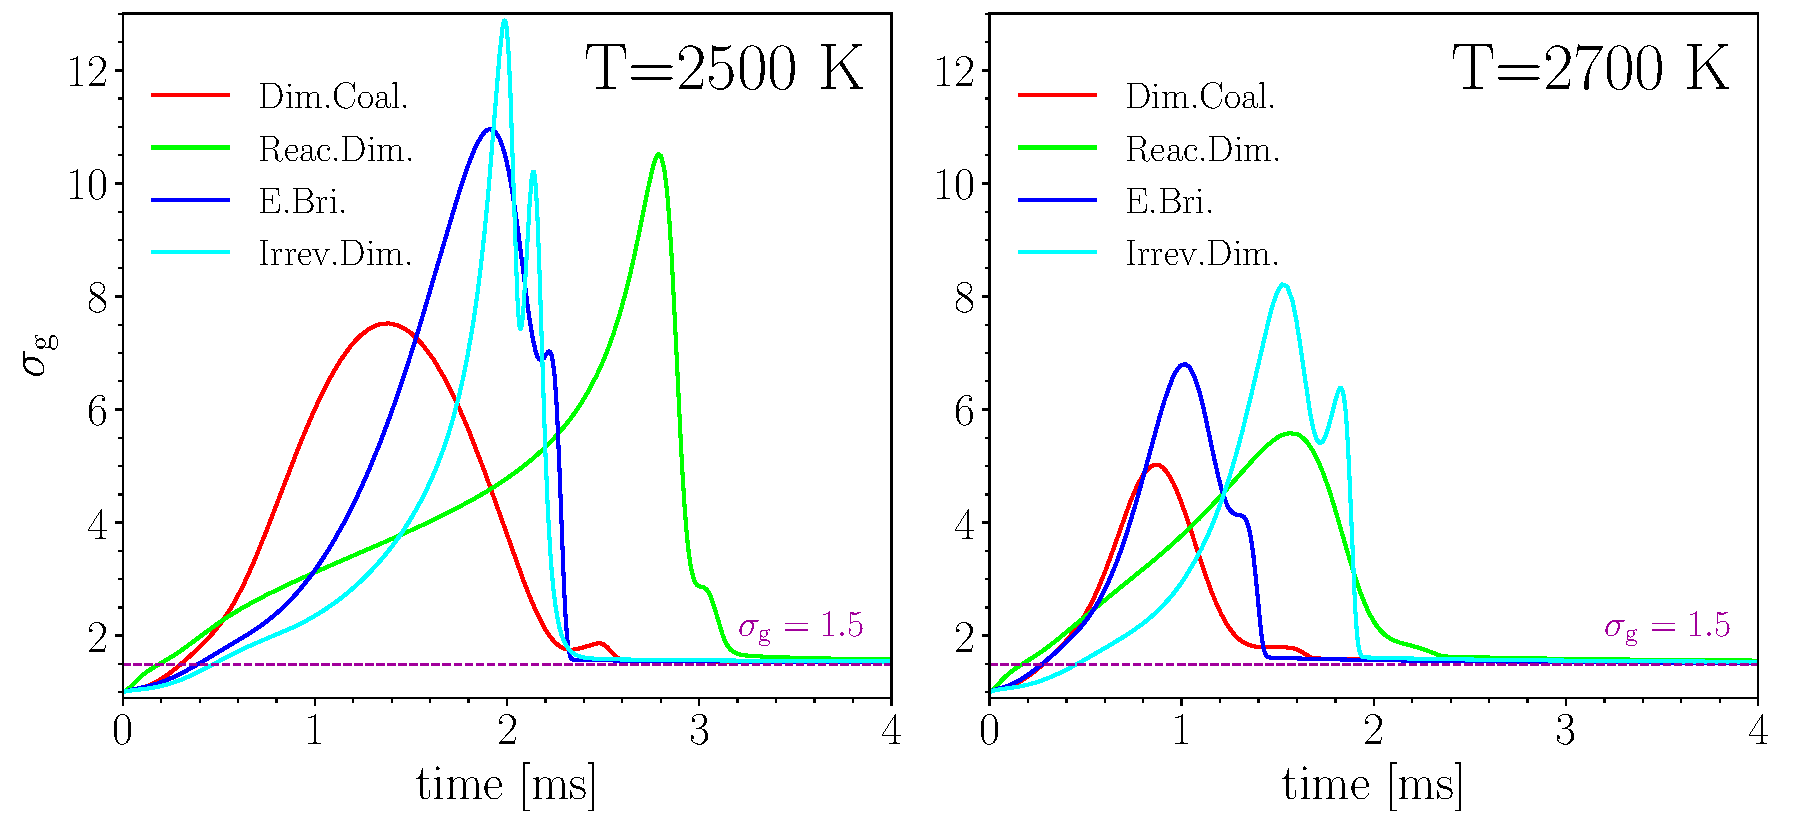
\includegraphics[width=0.8\textwidth]{Figures/Results/Shocktube/Agafonov2016/10CH4/sigma_time.pdf}
	\caption{The temperature dependence of standard geometric deviation of mobility diameter, $\mathrm{\sigma_{g}}$ during pyrolysis of 10\%~$\mathrm{CH_4}$-Ar at T=2500 K (left pane) and T=2700 K (right pane)}
	\label{fig:shocktubesigmatime} 
\end{figure}
